\chapter{Minimax}

Minimax é um algoritmo que visa minimizar a perda máxima, isto é, dentre
o pior caso de cada possível decisão aquele que levar ao menor prejuízo.
Originalmente formulado para um jogo de soma zero de dois jogadores, o Minimax
já foi estendido para jogos mais complexos e decisões gerais em situações de
incerteza.

% TODO: definir o que é A, B e H
O princípio do minimax se aplica a um jogo $\Gamma=\langle A,B,H\rangle$ se a
equação~\ref{eq:req} for satisfeita, isto é, se existe uma valoração $v$ para o
jogo e uma estratégia ótima para ambos jogadores.
\cite{hazewinkel2002encyclopaedia}

\begin{gather}
  v=\max_{a\in A}\min_{b\in B}H(a,b)=\min_{b\in B}\max_{a\in A}H(a,b)\label{eq:req}
\end{gather}

\section{Exemplo}

A figura~\ref{fig:minimax-tree} exemplifica uma árvore de decisão usando esse
método.

\begin{figure}[ht]
  \centering
  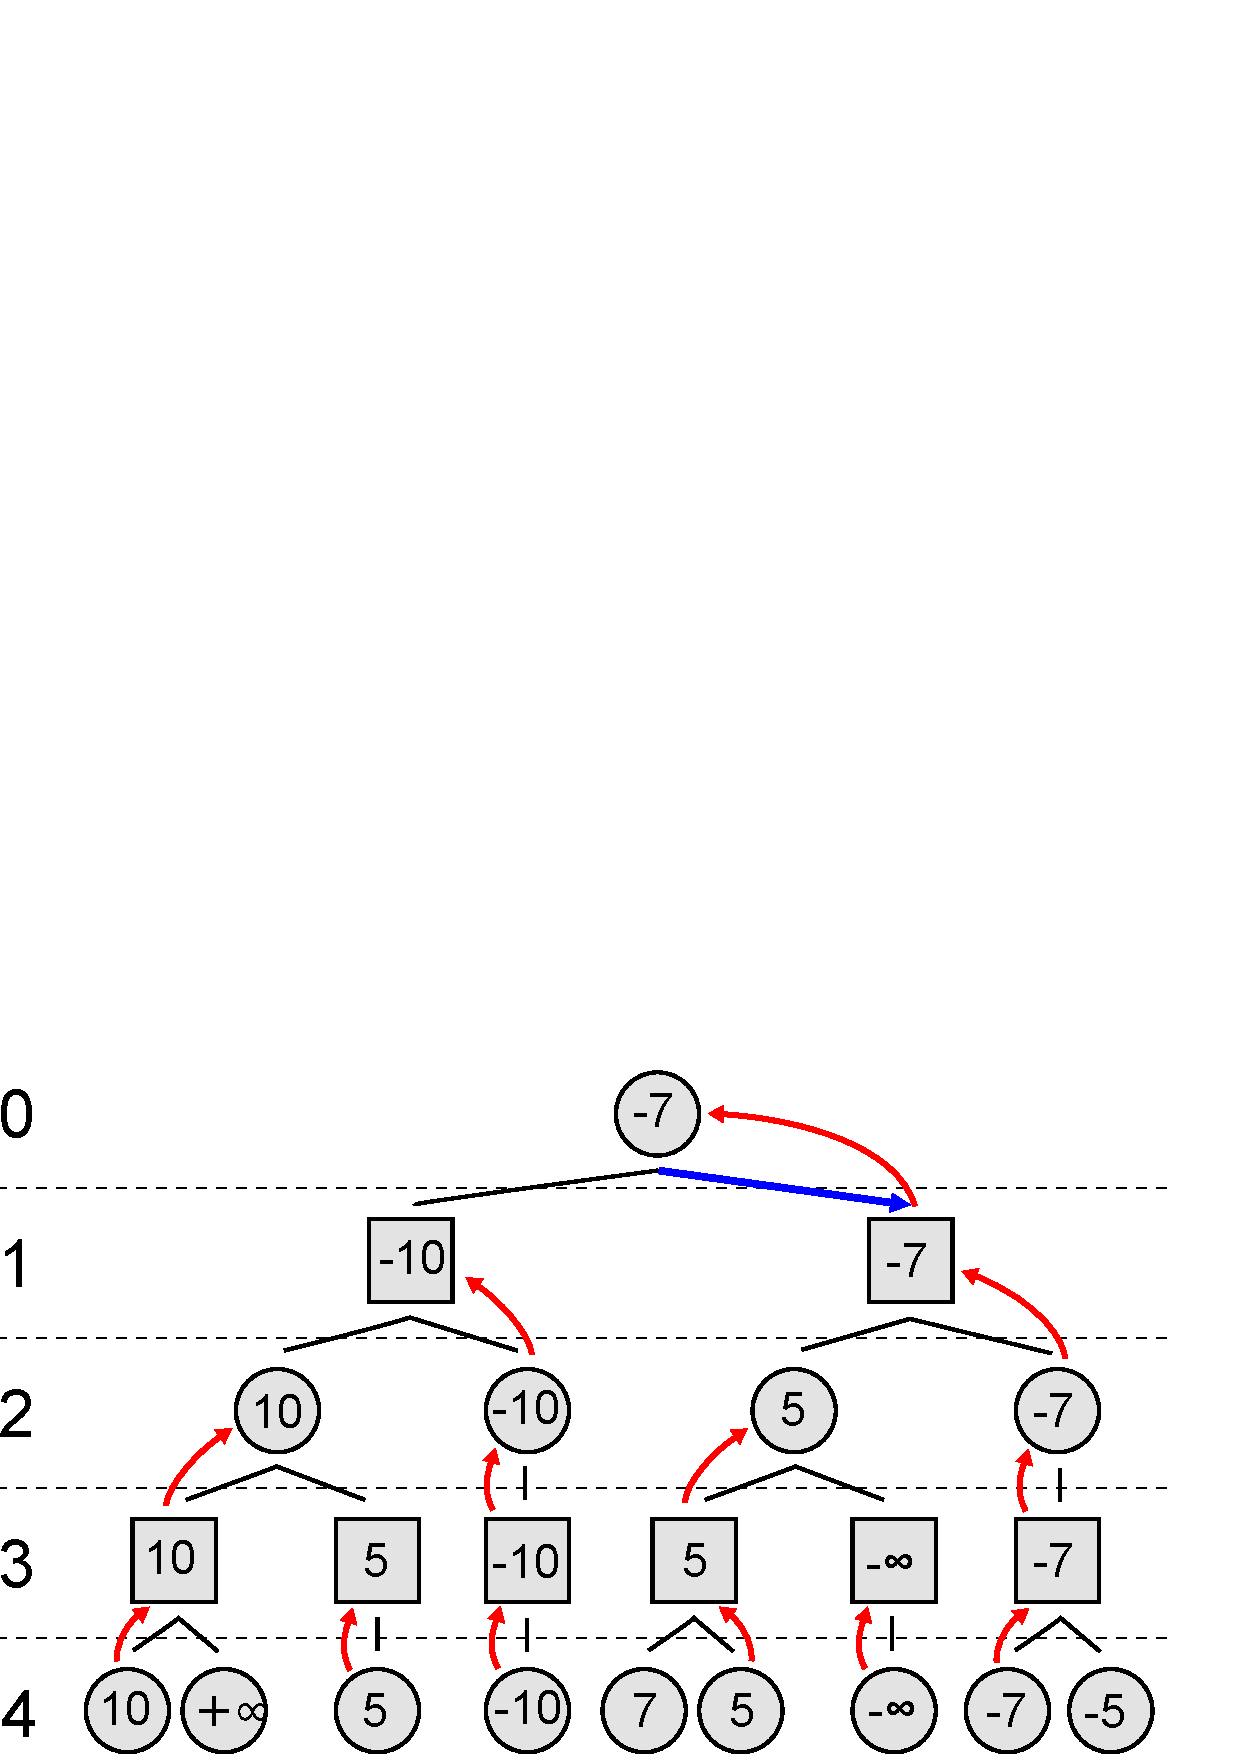
\includegraphics[width=0.7\linewidth]{minimax-tree}
  \caption{Exemplo de árvore de decisão com Minimax.}\label{fig:minimax-tree}
\end{figure}

% TODO: explicar através de uma exemplo
% TODO: explicar funcionamento
% TODO: Mostrar pseudo código

% vim: tw=80 et ts=2 sw=2 sts=2
